\documentclass[10pt,a4paper]{article}
\usepackage[utf8]{inputenc}
\usepackage{amsmath}
\usepackage{amsfonts}
\usepackage{amssymb}
\usepackage{graphicx}
\usepackage{enumerate}
\begin{document}

\section{Set Theory}

To demystify mathematics consider
\begin{enumerate}[(i)]
\item What is a theorem?
\item What is a proof?
\end{enumerate}
What if we don't know the answer?

To begin we need
\begin{enumerate}[(a)]
\item an example(s)
\item a nearly related concept
\end{enumerate}


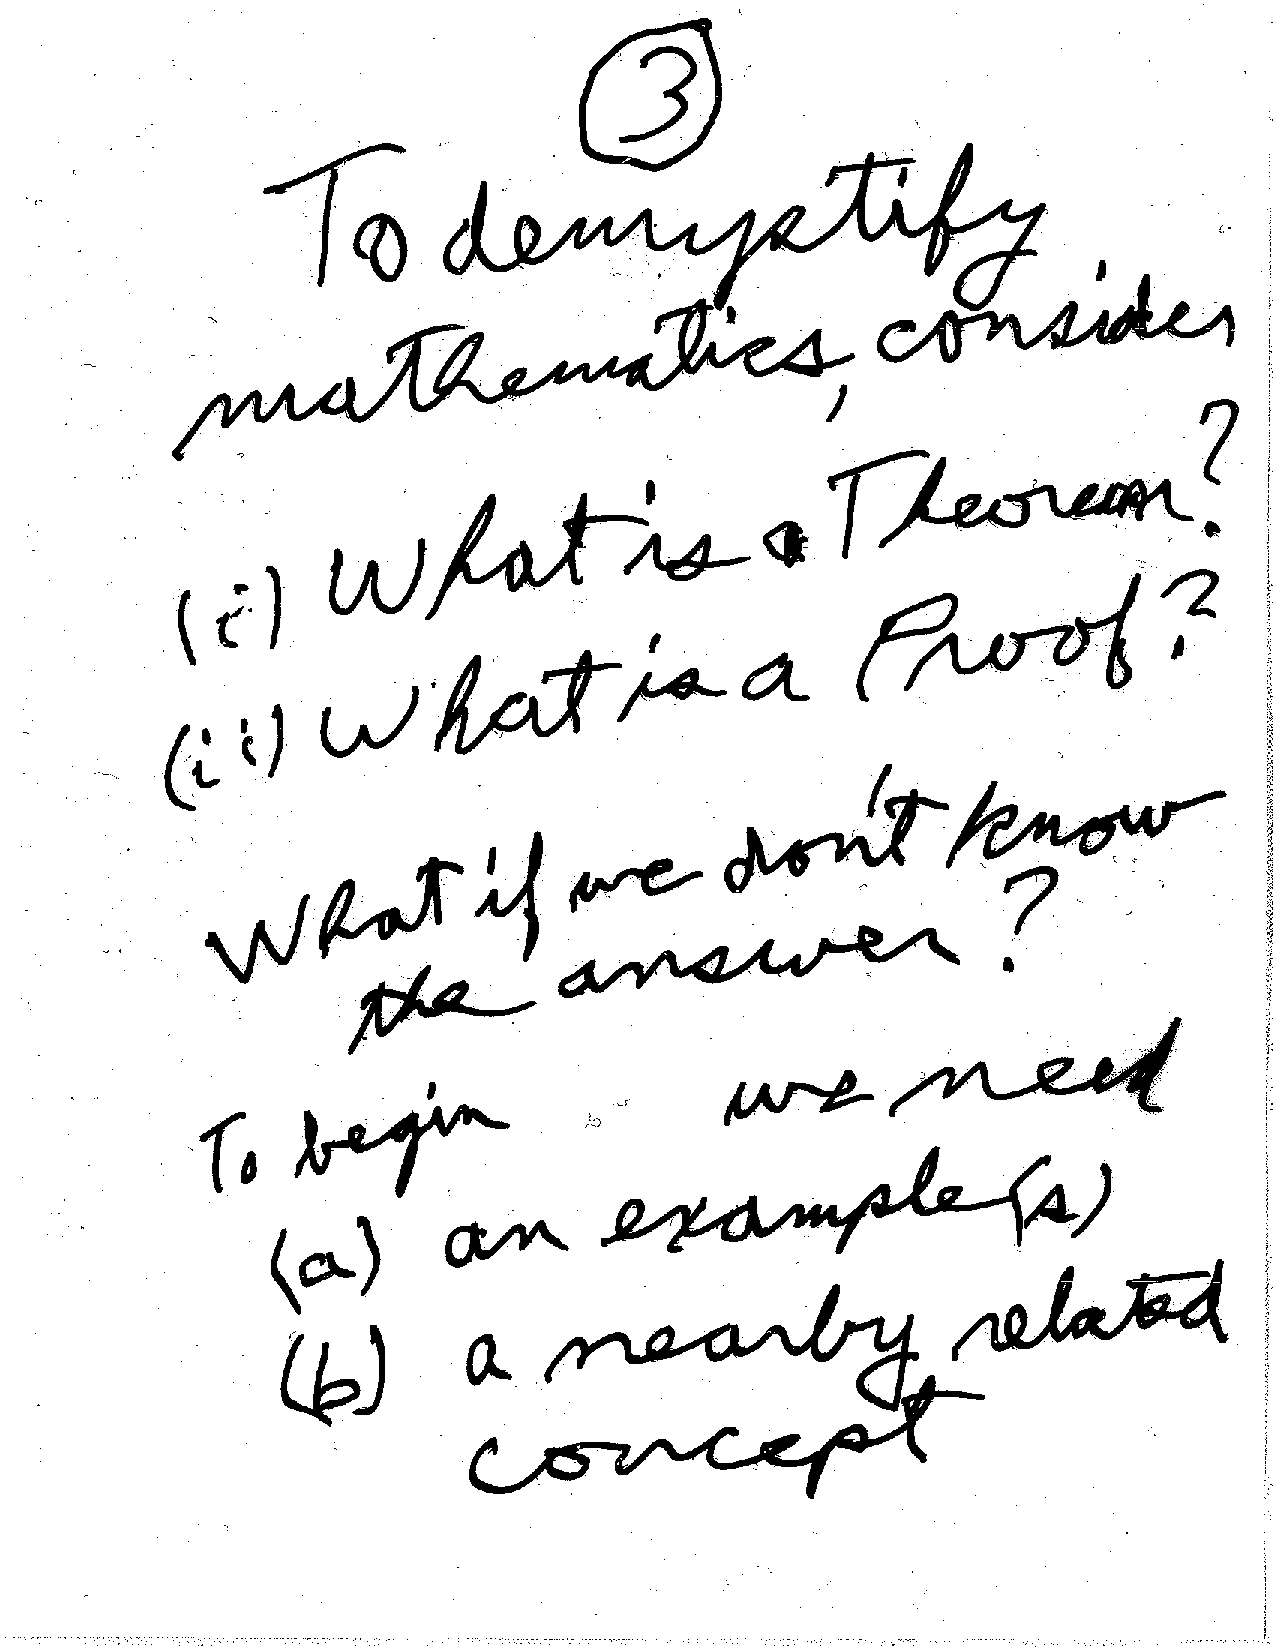
\includegraphics[scale=.5]{Pages/ST_3}

\newpage

Related Concept: Greek Syllogism

\underline{example:}
\begin{enumerate}
\item All men are mortal.
\item Socrates is a man.
\item Therefore, Socrates must die. 
\end{enumerate}

To analyze, recast in set theoretic terms via Venn Diagram.

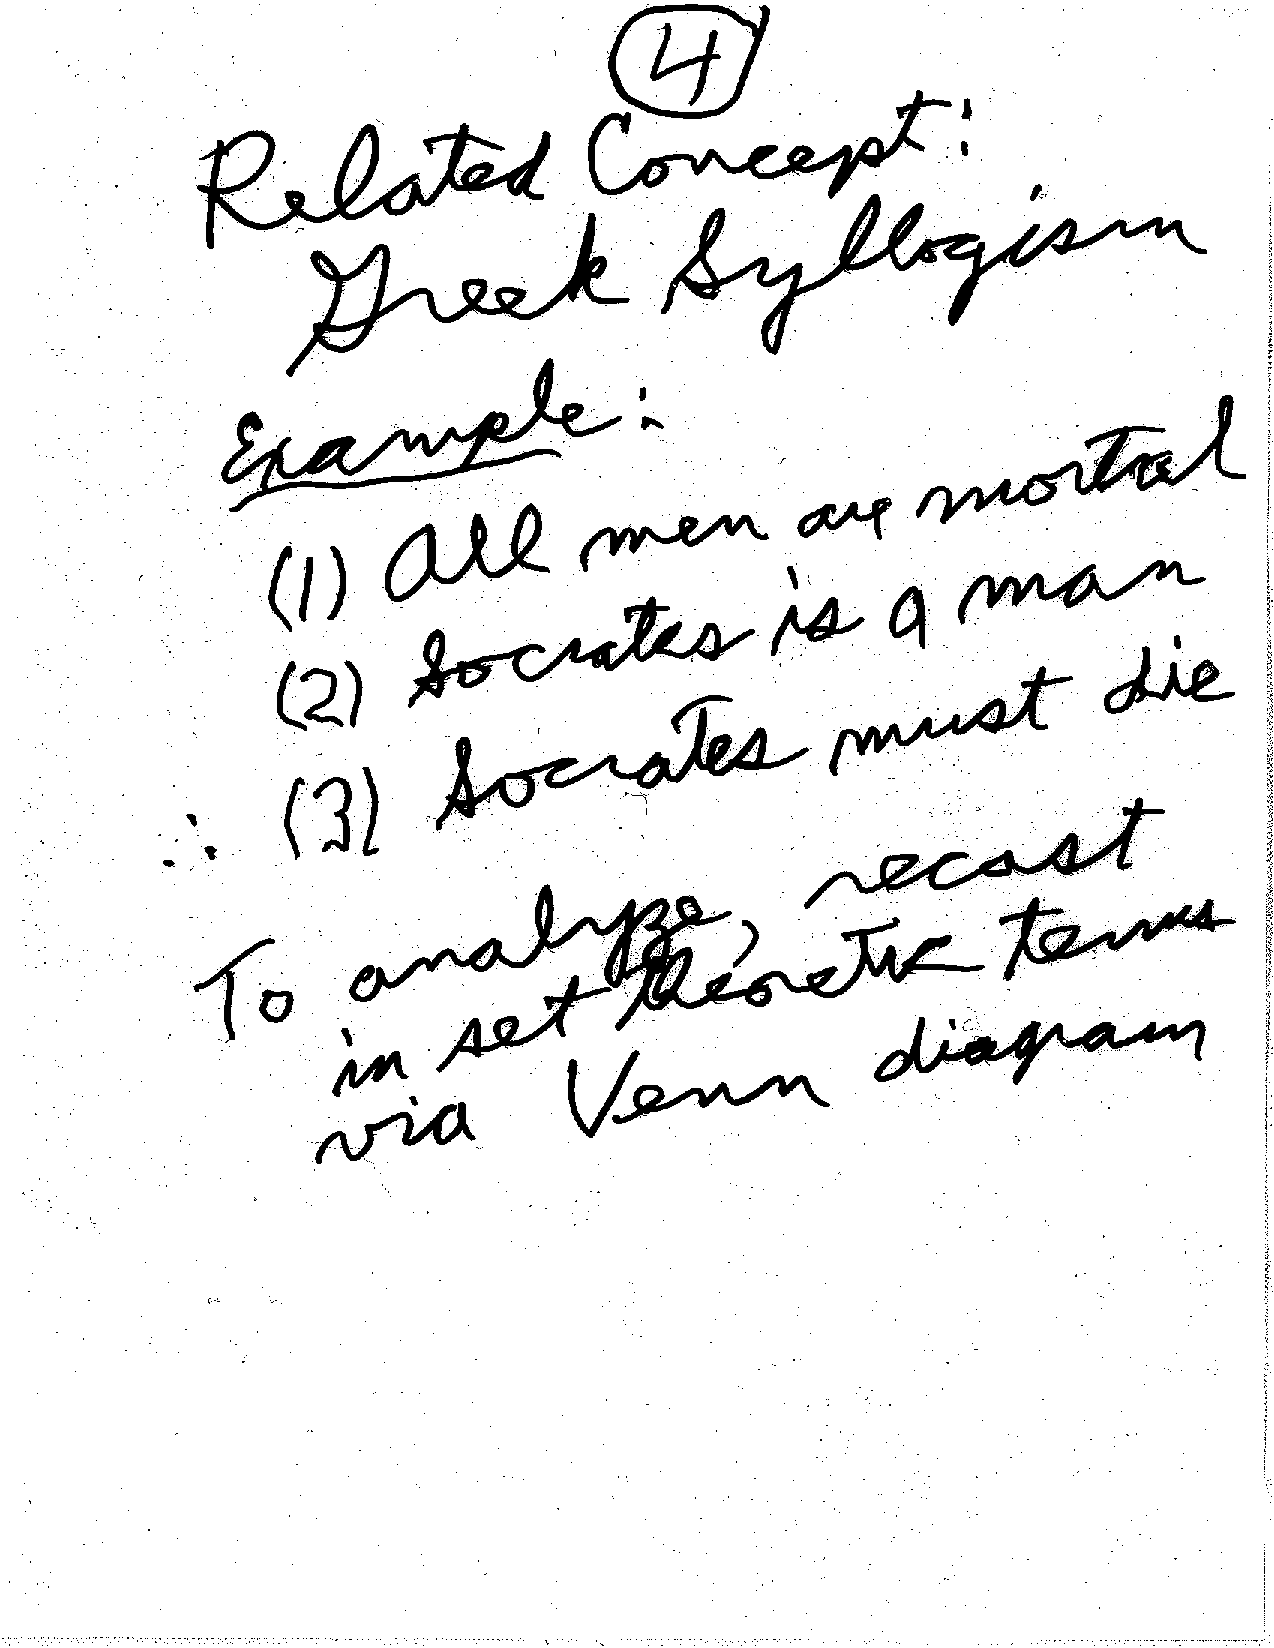
\includegraphics[scale=.5]{Pages/ST_4}

\newpage

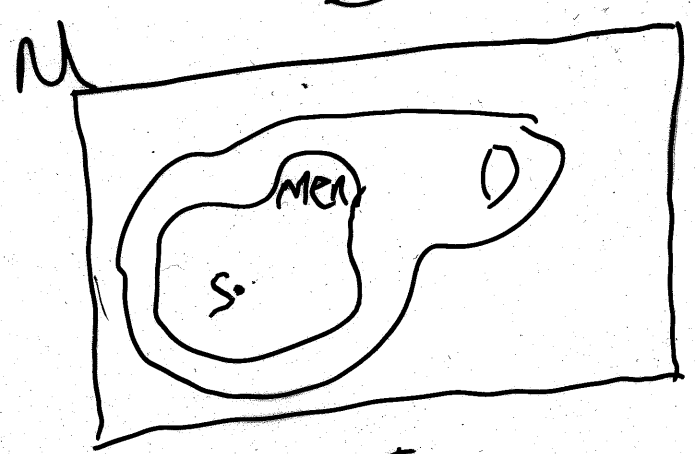
\includegraphics[scale=.2]{Pages/ST_5_im1}

$S$: Socrates\\
$M$: Set of Men\\
$D$: Things that will die\\
$\mathcal{U}$: Things on Earth

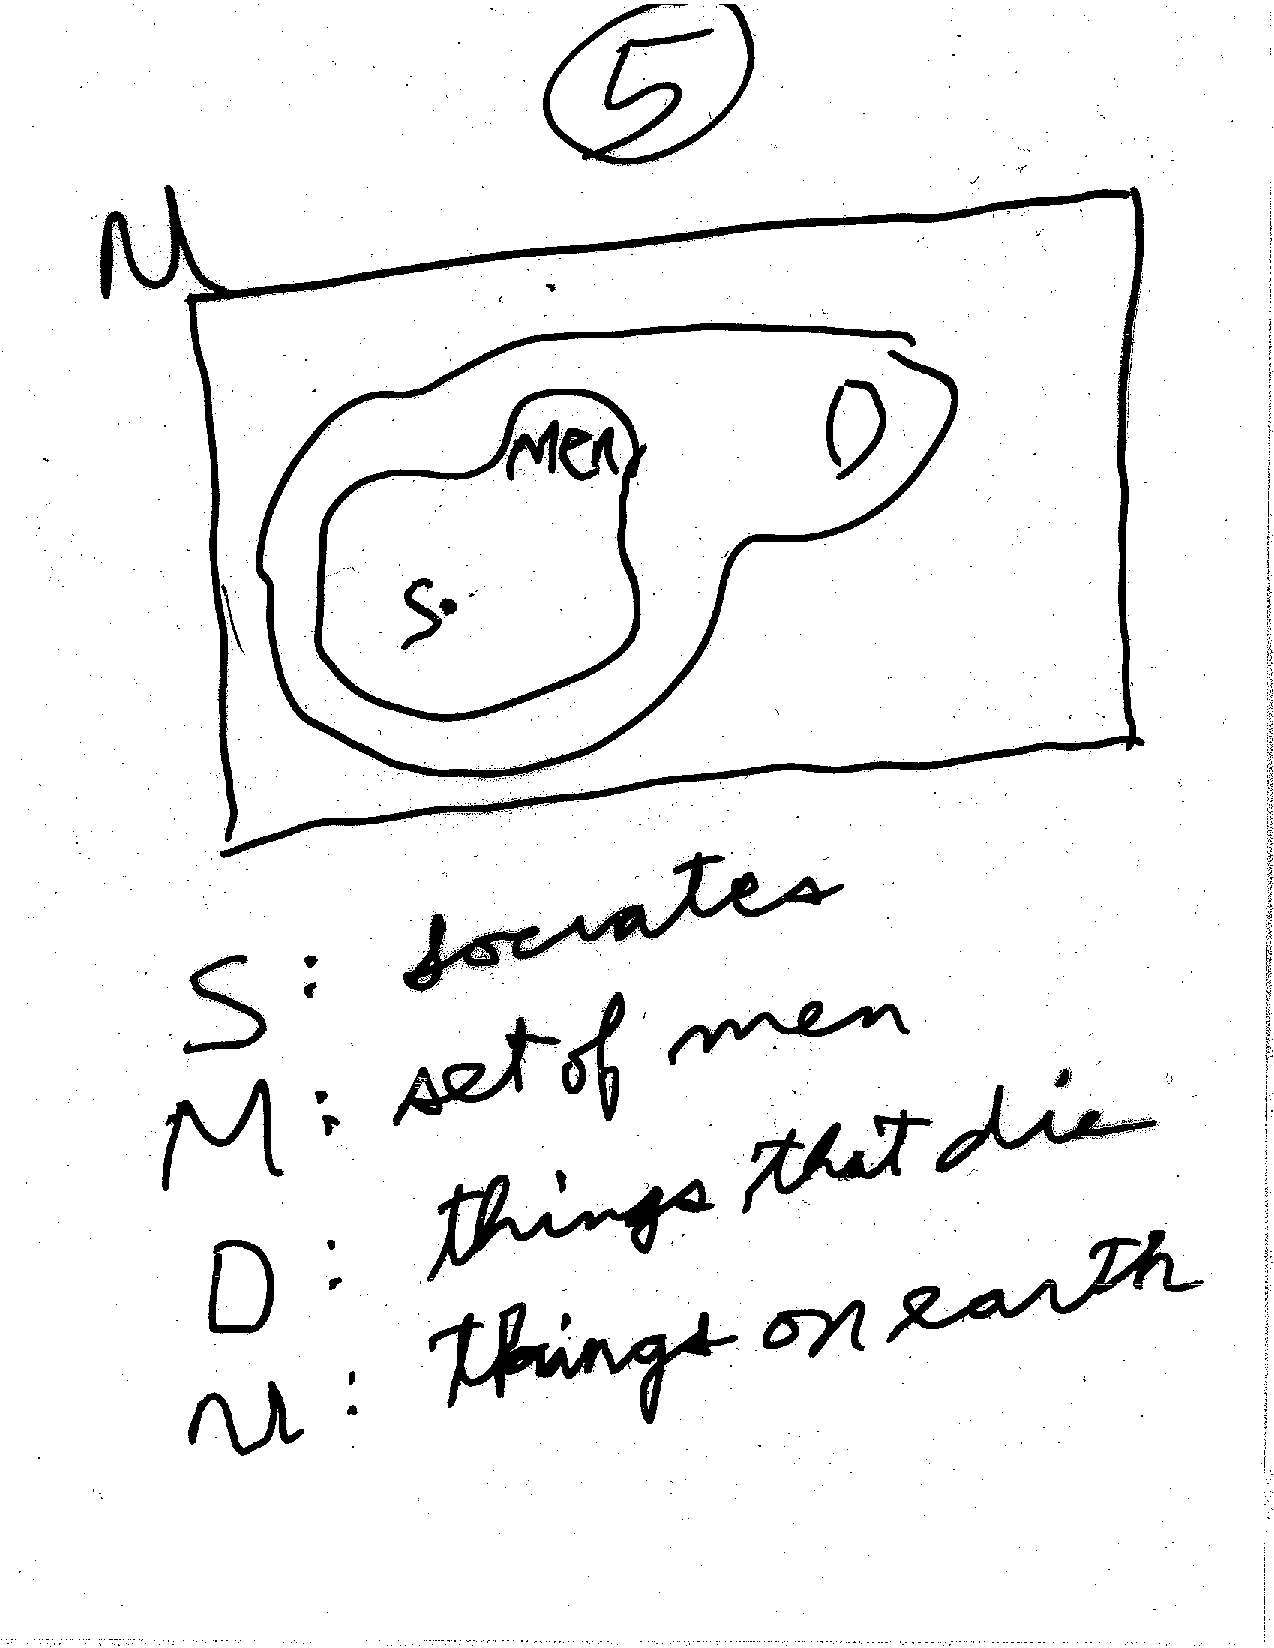
\includegraphics[scale=.5]{Pages/ST_5} 



%Zack: Pages 6,7,8,19,20

%Jack: 21, 9, 10, 11

%Koka: Pages 13, 13A, 22 ,22A, 22B


\section{Generate $\mathbb{N}$}


%Ruth: Pages L4A-L4G



\newpage

\section{From $\mathbb{Z}$ to $\mathbb{R}$ via ordering}
%Jazz: ZR1-ZR5

%Kyler: ZR6 - ZR10

%Preethika: ZR11-ZR14
What do the elements of $\mathbb{R}$ look like? 
\\On the number line they look like

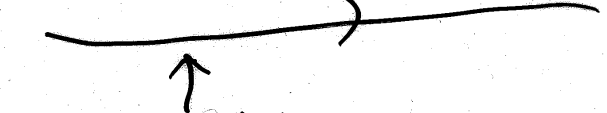
\includegraphics[scale=.5]{Pages/ZR_11_im1}
\\This set of dynamic rationals
\\How can we characterize them?

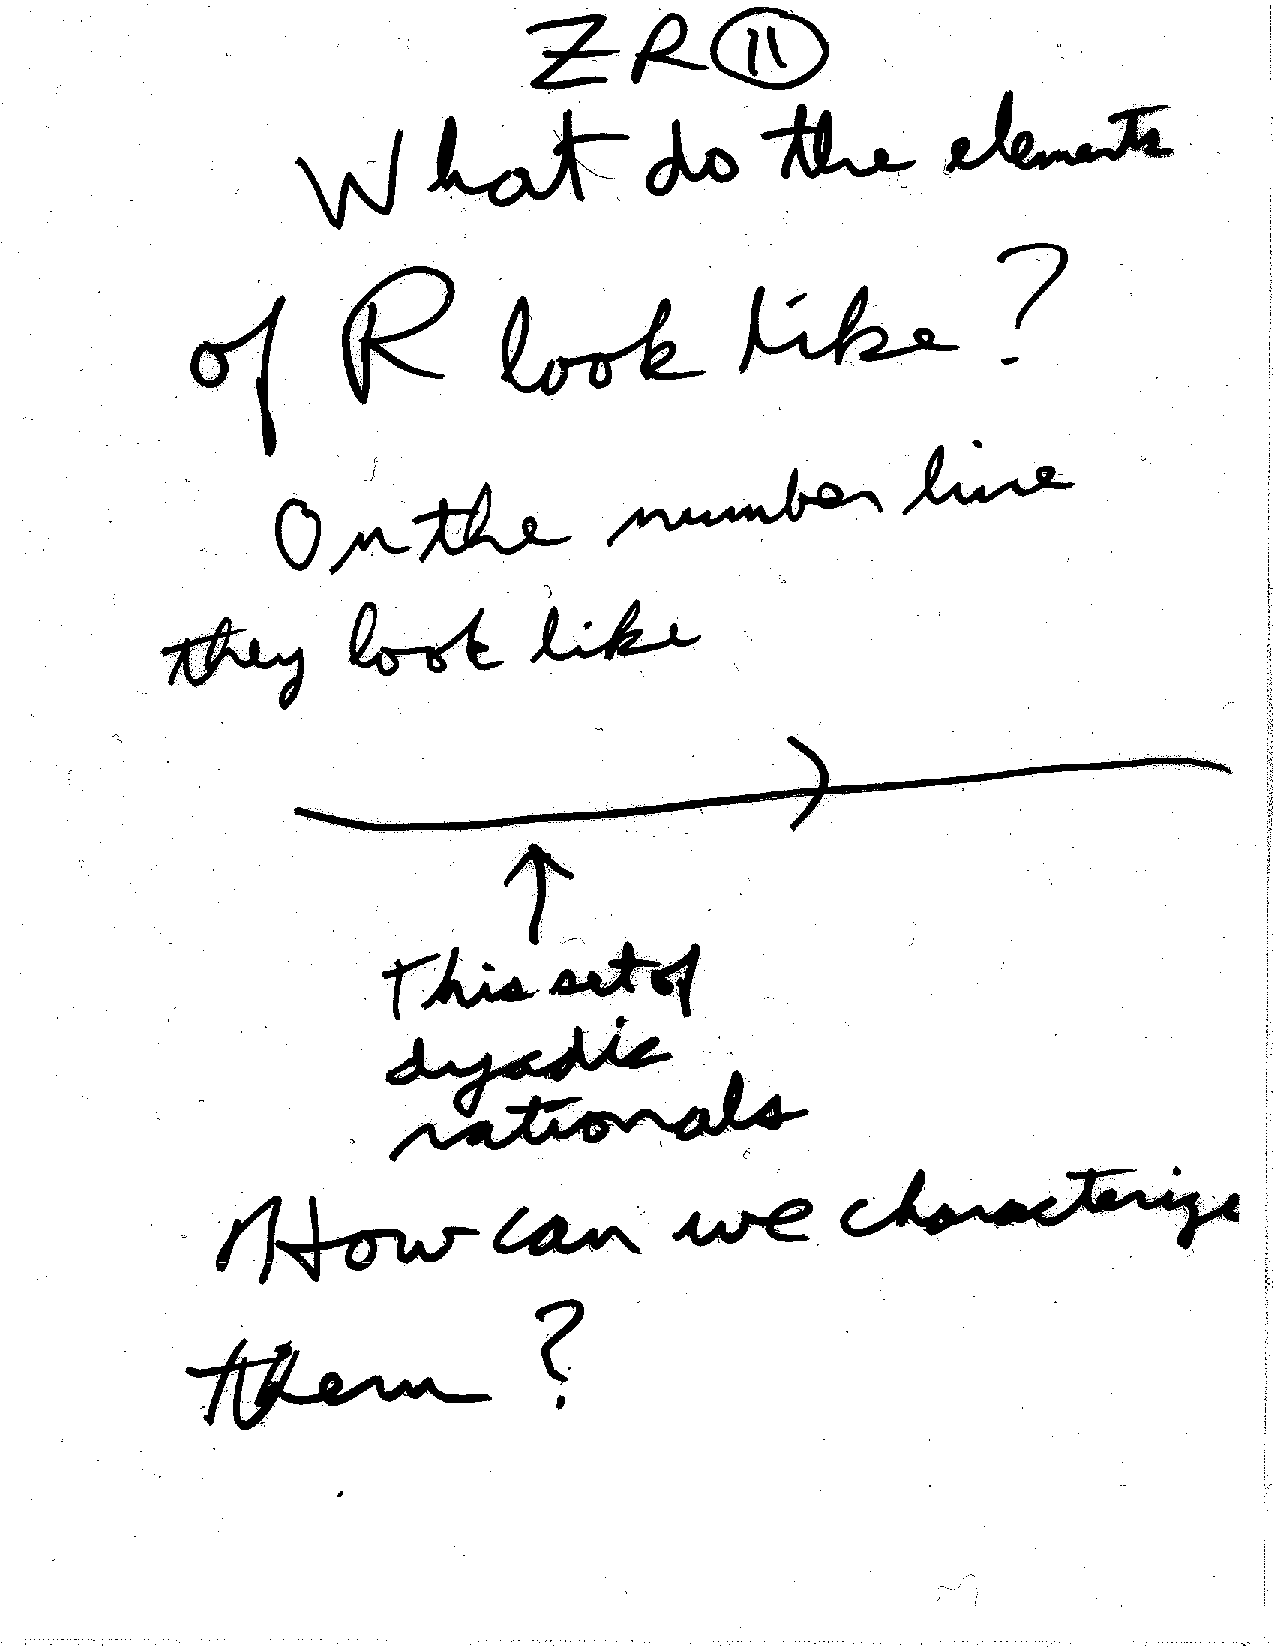
\includegraphics[scale=.5]{Pages/ZR_11}

\newpage

\underline{Therom} $B \in \mathbb{R}$ iff
\begin{enumerate}[(i)] 
\item $\phi \subsetneq B \subsetneq \mathbb{Z}_{(\infty)}$ 
\item If $b \in B$ and $a \in \mathbb{Z}_{(\infty)}$ with $a <_\infty b$ then $a \in B$
\item If $b \in B$ 
\\ $\exists b' \in B$ s.t
\\ $b <_\infty b'$

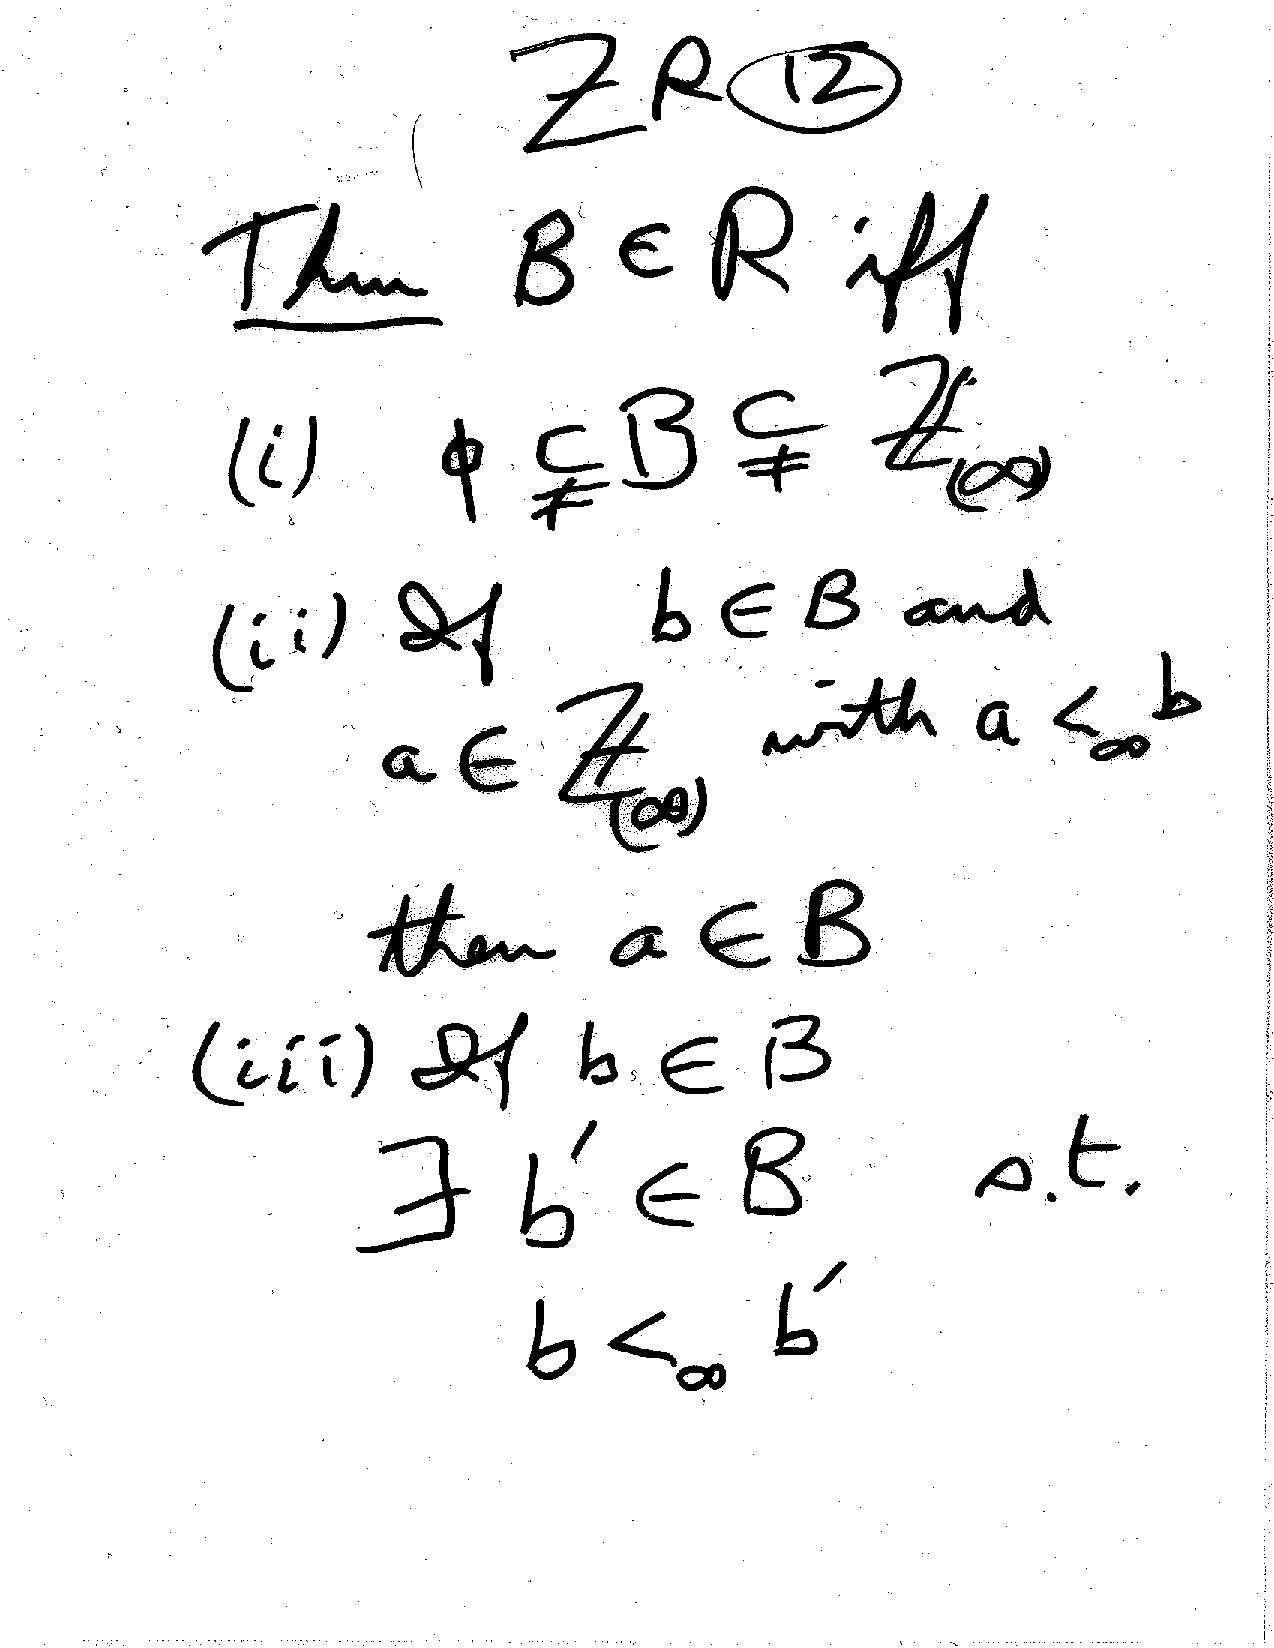
\includegraphics[scale=.5]{Pages/ZR_12}
\end{enumerate}

\newpage

$\underline{Pf:}^{(\Rightarrow)}$ Spse $B \in \mathbb{R}$
\\ $\exists$ non-entry $A \underline{\subset} \mathbb{Z}_{(\infty)}$
\\ s.t $$B=\bigcup_{a \in A} \mathcal{L}_a$$
\\ We are given that
\\ $B \neq \emptyset$ and $B \neq \mathbb{Z}_{(\infty)}$ 
\begin{enumerate}[(ii)] 
\item Spse $b \in B$
\\ and $b_o <_\infty b$ with $b_o \in \mathbb{Z}_{(\infty)}$
\\ $\exists a \in A: b \in \mathcal{L}_a$
\\hence $b_o \in \mathcal{L}_a$
\\ so $b_o \in B$
\item holds for -------$>$ $\mathcal{L}_a$ so (iii) holds. 

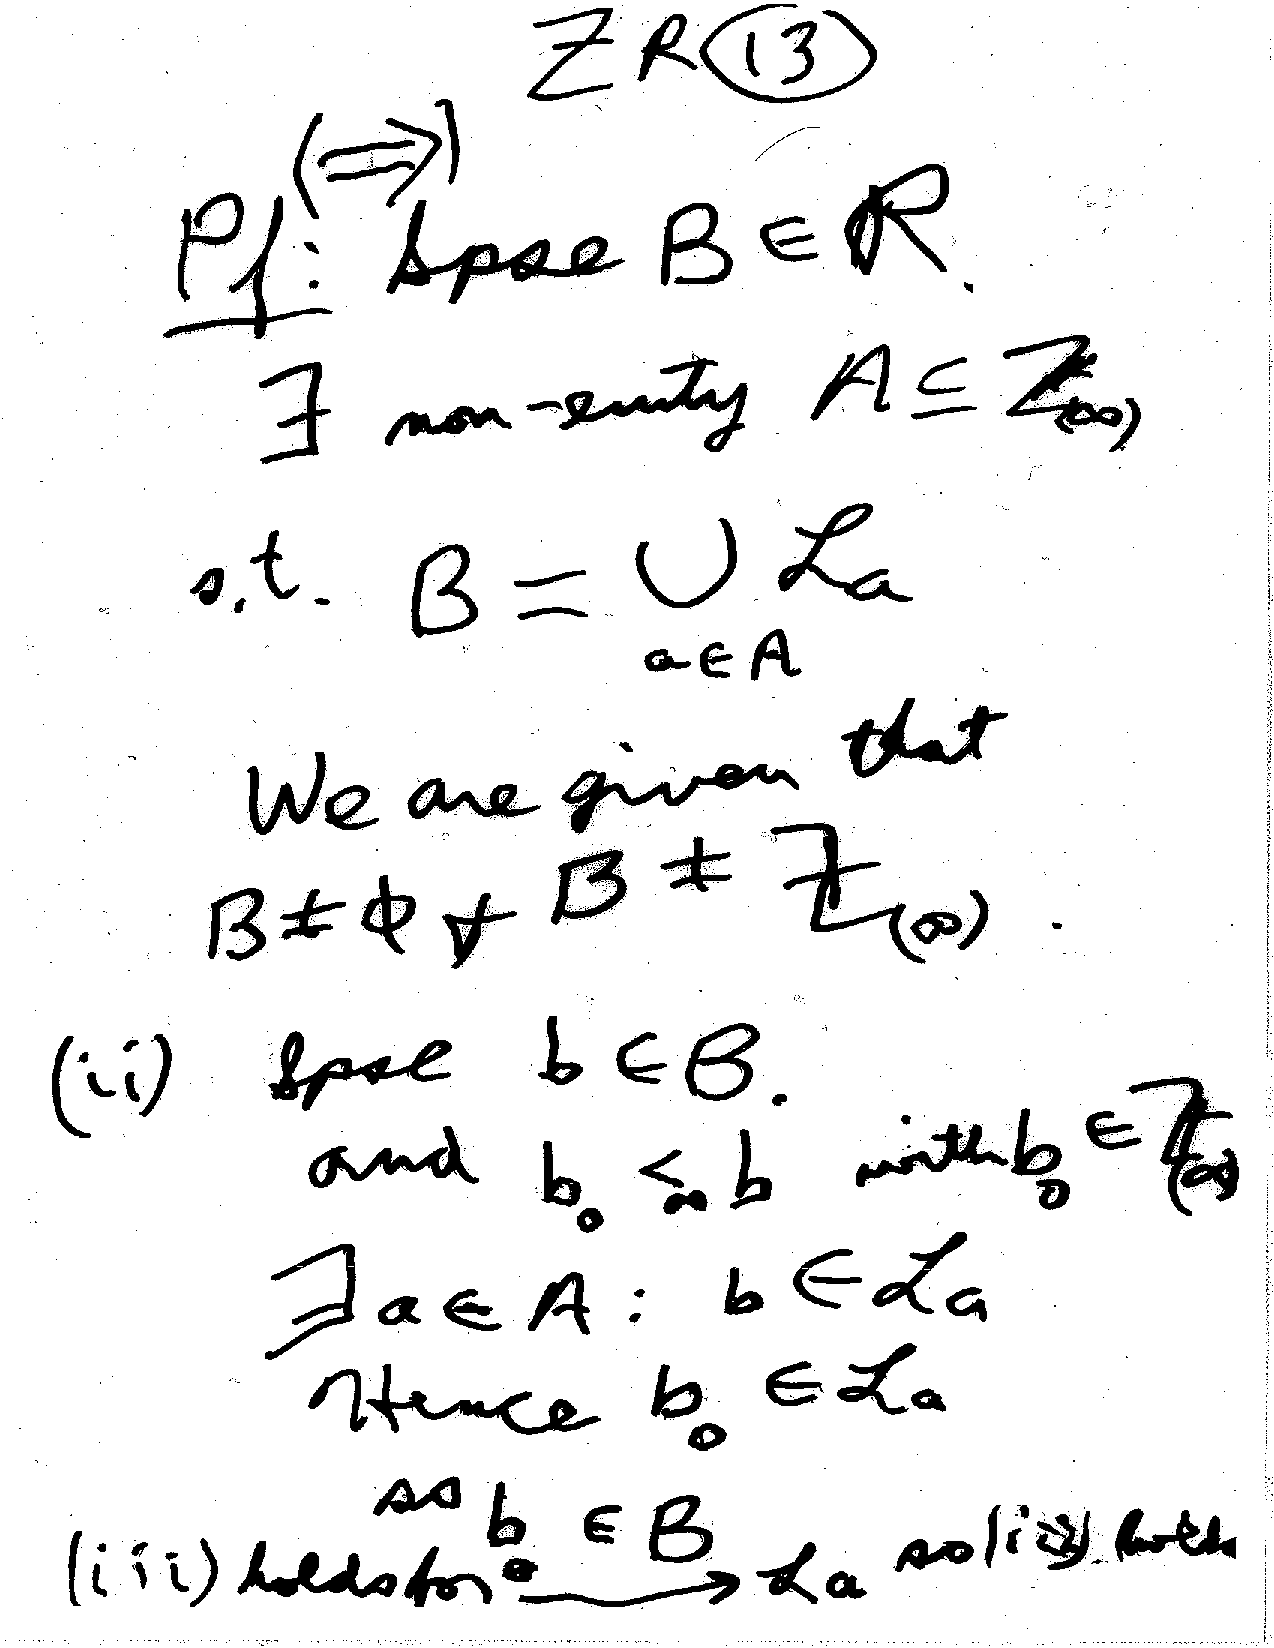
\includegraphics[scale=.5]{Pages/ZR_13}

\newpage
($\Leftarrow$)Conversely,
\\Spse B satisfies (i),(ii),(iii)
\\Let $A=B$
\\$\emptyset \subsetneq A \subsetneq \mathbb{Z}_{(\infty)}$
\\Claim $$B=\bigcup_{a \in A} \mathcal{L}_a $$ 
\\Clearly $ \bigcup \mathcal{L}_a \underline{\subset} B$ (Why?)
\\Take away $b \in B$. 
\\ $\exists b' >_\infty b$ s.t $b' \in B$
\\ $b \in \mathcal{L}_b{'}$ so
\\ $$B \underline{\subset} \bigcup_{a \in A} \mathcal{L}_a$$ qed

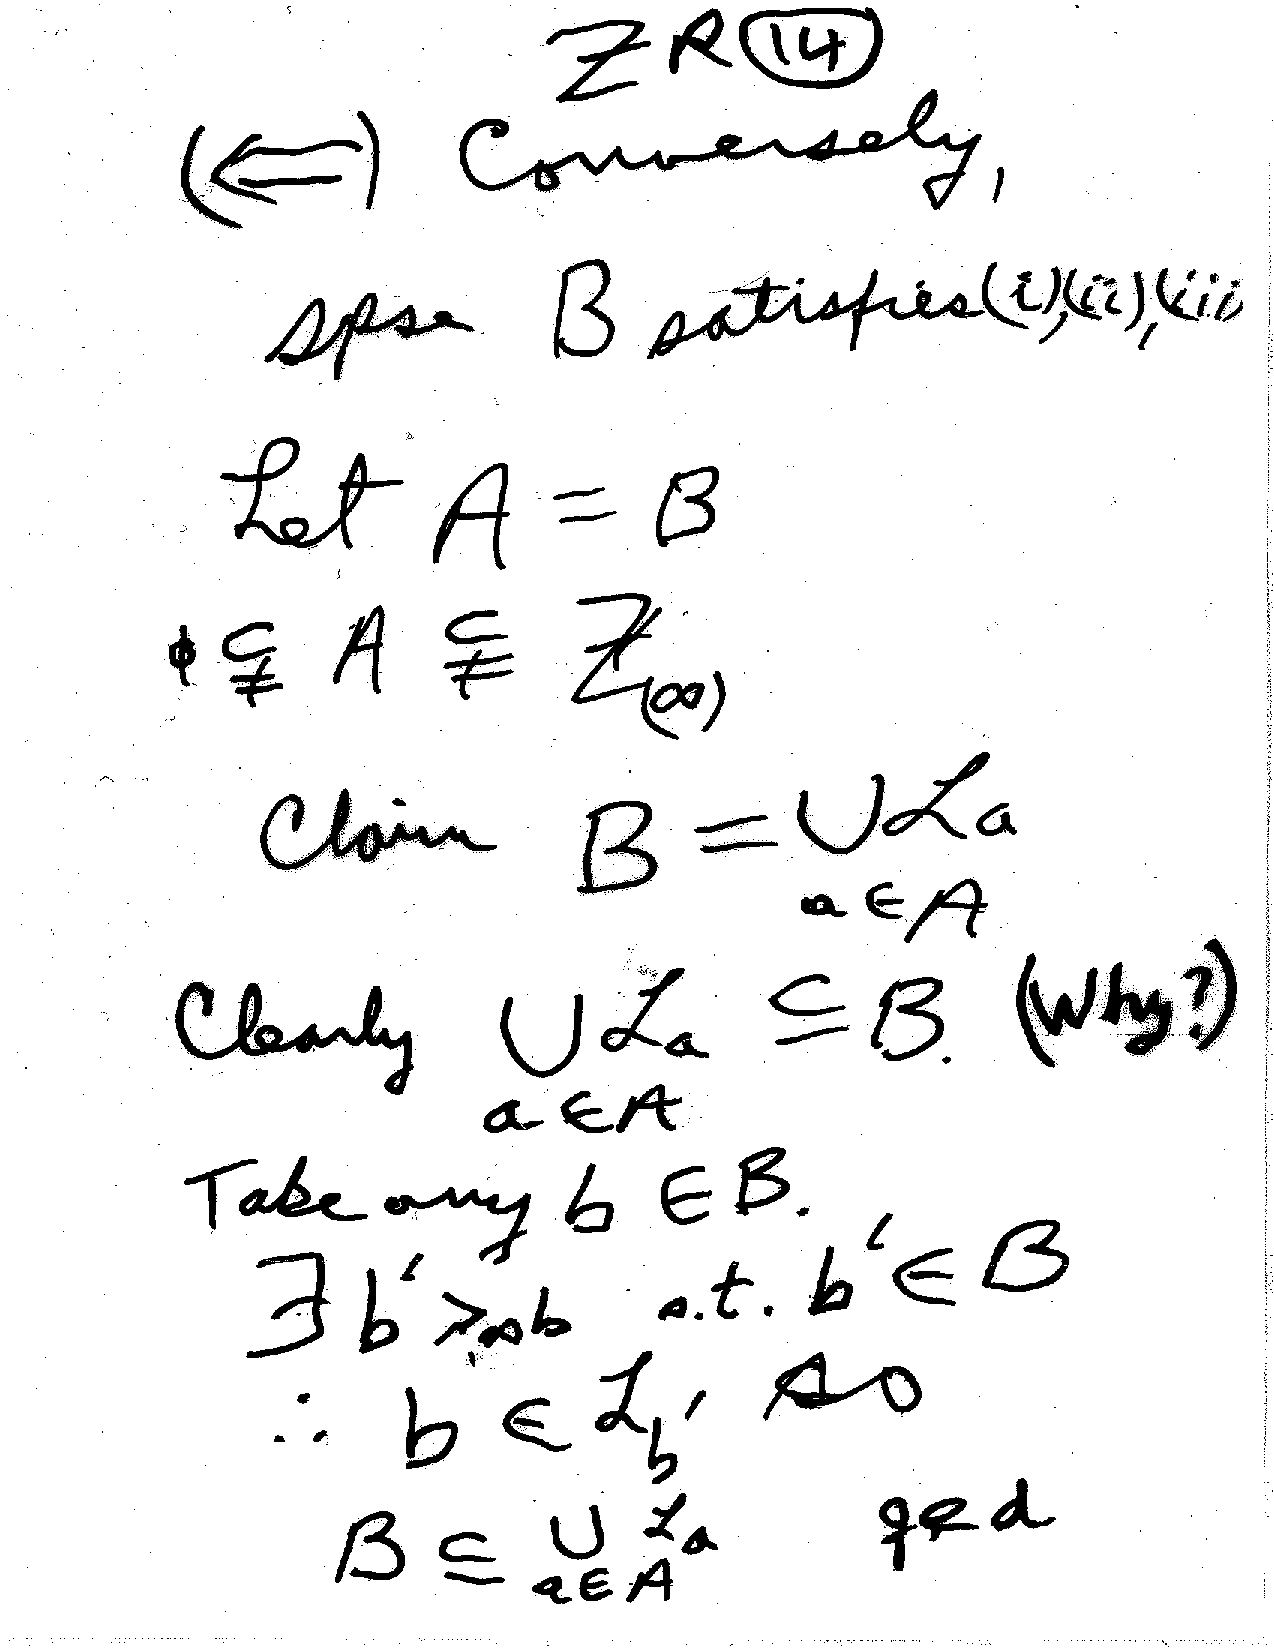
\includegraphics[scale=.5]{Pages/ZR_14}

\end{enumerate}

\section{Sequence and Limits}

%Aaron: First 2 pages and 48-50

%Hamza: 51-52B

\section{Limit and Convergence}

%Joe: 50-51

%Quinten: 52-53

%Farishta: 53A-54A

\section{Infinite Series}

%Sukhreet: IS1 - IS 7

%Matthew: IS8 - IS15

%Will: IS16 - IS23

%Rebecca: IS24 - IS32

%Maady: IS33 - IS42

\section{Metric Spaces Part 1}

%Travis: M1 - M5

%Jerome: M6- M10



\section{Metric Spaces Part 2}


%Bryant: M1-M7

%Reshma: M8-M14

%Ethan: M15-M21




\end{document}